% Options for packages loaded elsewhere
% Options for packages loaded elsewhere
\PassOptionsToPackage{unicode}{hyperref}
\PassOptionsToPackage{hyphens}{url}
\PassOptionsToPackage{dvipsnames,svgnames,x11names}{xcolor}
%
\documentclass[
  spanish,
  letterpaper,
  DIV=11,
  numbers=noendperiod]{scrartcl}
\usepackage{xcolor}
\usepackage{amsmath,amssymb}
\setcounter{secnumdepth}{-\maxdimen} % remove section numbering
\usepackage{iftex}
\ifPDFTeX
  \usepackage[T1]{fontenc}
  \usepackage[utf8]{inputenc}
  \usepackage{textcomp} % provide euro and other symbols
\else % if luatex or xetex
  \usepackage{unicode-math} % this also loads fontspec
  \defaultfontfeatures{Scale=MatchLowercase}
  \defaultfontfeatures[\rmfamily]{Ligatures=TeX,Scale=1}
\fi
\usepackage{lmodern}
\ifPDFTeX\else
  % xetex/luatex font selection
\fi
% Use upquote if available, for straight quotes in verbatim environments
\IfFileExists{upquote.sty}{\usepackage{upquote}}{}
\IfFileExists{microtype.sty}{% use microtype if available
  \usepackage[]{microtype}
  \UseMicrotypeSet[protrusion]{basicmath} % disable protrusion for tt fonts
}{}
\makeatletter
\@ifundefined{KOMAClassName}{% if non-KOMA class
  \IfFileExists{parskip.sty}{%
    \usepackage{parskip}
  }{% else
    \setlength{\parindent}{0pt}
    \setlength{\parskip}{6pt plus 2pt minus 1pt}}
}{% if KOMA class
  \KOMAoptions{parskip=half}}
\makeatother
% Make \paragraph and \subparagraph free-standing
\makeatletter
\ifx\paragraph\undefined\else
  \let\oldparagraph\paragraph
  \renewcommand{\paragraph}{
    \@ifstar
      \xxxParagraphStar
      \xxxParagraphNoStar
  }
  \newcommand{\xxxParagraphStar}[1]{\oldparagraph*{#1}\mbox{}}
  \newcommand{\xxxParagraphNoStar}[1]{\oldparagraph{#1}\mbox{}}
\fi
\ifx\subparagraph\undefined\else
  \let\oldsubparagraph\subparagraph
  \renewcommand{\subparagraph}{
    \@ifstar
      \xxxSubParagraphStar
      \xxxSubParagraphNoStar
  }
  \newcommand{\xxxSubParagraphStar}[1]{\oldsubparagraph*{#1}\mbox{}}
  \newcommand{\xxxSubParagraphNoStar}[1]{\oldsubparagraph{#1}\mbox{}}
\fi
\makeatother


\usepackage{longtable,booktabs,array}
\newcounter{none} % for unnumbered tables
\usepackage{calc} % for calculating minipage widths
% Correct order of tables after \paragraph or \subparagraph
\usepackage{etoolbox}
\makeatletter
\patchcmd\longtable{\par}{\if@noskipsec\mbox{}\fi\par}{}{}
\makeatother
% Allow footnotes in longtable head/foot
\IfFileExists{footnotehyper.sty}{\usepackage{footnotehyper}}{\usepackage{footnote}}
\makesavenoteenv{longtable}
\usepackage{graphicx}
\makeatletter
\newsavebox\pandoc@box
\newcommand*\pandocbounded[1]{% scales image to fit in text height/width
  \sbox\pandoc@box{#1}%
  \Gscale@div\@tempa{\textheight}{\dimexpr\ht\pandoc@box+\dp\pandoc@box\relax}%
  \Gscale@div\@tempb{\linewidth}{\wd\pandoc@box}%
  \ifdim\@tempb\p@<\@tempa\p@\let\@tempa\@tempb\fi% select the smaller of both
  \ifdim\@tempa\p@<\p@\scalebox{\@tempa}{\usebox\pandoc@box}%
  \else\usebox{\pandoc@box}%
  \fi%
}
% Set default figure placement to htbp
\def\fps@figure{htbp}
\makeatother



\ifLuaTeX
\usepackage[bidi=basic,shorthands=off]{babel}
\else
\usepackage[bidi=default,shorthands=off]{babel}
\fi
\ifLuaTeX
  \usepackage{selnolig} % disable illegal ligatures
\fi


\setlength{\emergencystretch}{3em} % prevent overfull lines

\providecommand{\tightlist}{%
  \setlength{\itemsep}{0pt}\setlength{\parskip}{0pt}}



 


\usepackage{booktabs}
\usepackage{caption}
\usepackage{longtable}
\usepackage{colortbl}
\usepackage{array}
\usepackage{anyfontsize}
\usepackage{multirow}
\KOMAoption{captions}{tableheading}
\makeatletter
\@ifpackageloaded{caption}{}{\usepackage{caption}}
\AtBeginDocument{%
\ifdefined\contentsname
  \renewcommand*\contentsname{Tabla de contenidos}
\else
  \newcommand\contentsname{Tabla de contenidos}
\fi
\ifdefined\listfigurename
  \renewcommand*\listfigurename{Listado de Figuras}
\else
  \newcommand\listfigurename{Listado de Figuras}
\fi
\ifdefined\listtablename
  \renewcommand*\listtablename{Listado de Tablas}
\else
  \newcommand\listtablename{Listado de Tablas}
\fi
\ifdefined\figurename
  \renewcommand*\figurename{Figura}
\else
  \newcommand\figurename{Figura}
\fi
\ifdefined\tablename
  \renewcommand*\tablename{Tabla}
\else
  \newcommand\tablename{Tabla}
\fi
}
\@ifpackageloaded{float}{}{\usepackage{float}}
\floatstyle{ruled}
\@ifundefined{c@chapter}{\newfloat{codelisting}{h}{lop}}{\newfloat{codelisting}{h}{lop}[chapter]}
\floatname{codelisting}{Listado}
\newcommand*\listoflistings{\listof{codelisting}{Listado de Listados}}
\makeatother
\makeatletter
\makeatother
\makeatletter
\@ifpackageloaded{caption}{}{\usepackage{caption}}
\@ifpackageloaded{subcaption}{}{\usepackage{subcaption}}
\makeatother
\usepackage{bookmark}
\IfFileExists{xurl.sty}{\usepackage{xurl}}{} % add URL line breaks if available
\urlstyle{same}
% fallback for those not using the hyperref driver hyperxmp:
\makeatletter
\@ifundefined{xmpquote}{\newcommand{\xmpquote}[1]{#1}}{}
\makeatother
\hypersetup{
  pdftitle={Informe 1. Evaluación Regresión Lineal},
  pdfauthor={Emilia Barrientos Carrasco; Pablo Campos Abutridy},
  pdflang={es},
  colorlinks=true,
  linkcolor={blue},
  filecolor={Maroon},
  citecolor={Blue},
  urlcolor={Blue},
  pdfcreator={LaTeX via pandoc}}


\title{Informe 1. Evaluación Regresión Lineal}
\usepackage{etoolbox}
\makeatletter
\providecommand{\subtitle}[1]{% add subtitle to \maketitle
  \apptocmd{\@title}{\par {\large #1 \par}}{}{}
}
\makeatother
\subtitle{Diplomado en Estadística, mención Métodos Estadísticos}
\author{Emilia Barrientos Carrasco \and Pablo Campos Abutridy}
\date{lunes 3 de agosto de 2026}
\begin{document}
\maketitle


\section{Pregunta 1. Mejor MRLS basado en variables
metereológicas.}\label{pregunta-1.-mejor-mrls-basado-en-variables-metereoluxf3gicas.}

Inicialmente, se calculó una matriz de correlación para cada una de las
variables de la base de datos, con el fin de explorar la intensidad y
dirección de sus asociaciones lineales (ver Tabla~\ref{tbl-corr-df} ). A
partir de este análisis, se observó que la variable \emph{PM2.5}
presentó una correlación de mayor magnitud con las variables
metereológicas \emph{TMin} (-0,63), \emph{TProm} (-0,62) y \emph{Viento}
(-0,60). Así, se constituyeron como candidatas para explicar la
variabilidad del material particulado (\emph{PM2.5}).

Luego, se ajustaron cinco modelos de regresión lineal simple con el
objetivo de estimar el nivel de \emph{PM2.5} a partir de cada uno de los
predictores meteorológicos (\emph{Viento}, \emph{TProm}, \emph{TMin},
\emph{TMax} y \emph{Humed}). Estos modelos se compararon considerando su
R² y la significancia global de cada uno (estadístico F y su valor-p).
Así, se seleccionó el Modelo 3 (predictor \emph{TMin}) porque cuenta con
la mayor capacidad explicativa (R² = 0,3921), el menor error estándar
residual (12,87) y el mayor estadístico F (101,9).

\begin{table}[H]

\caption{\label{tbl-mod-met}Comparación de MRLS con predictores
meteorológicos}

\centering{

\fontsize{8.0pt}{9.0pt}\selectfont
\begin{tabular*}{0.8\linewidth}{@{\extracolsep{\fill}}lccccc}
\toprule
  & Modelo 1 & Modelo 2 & Modelo 3 & Modelo 4 & Modelo 5 \\ 
\midrule\addlinespace[2.5pt]
(Intercept) & 48.033*** & 58.000*** & 45.418*** & 56.285*** & -10.774 \\ 
 & (2.865) & (3.671) & (2.468) & (5.389) & (6.414) \\ 
Viento & -26.767*** &  &  &  &  \\ 
 & (2.822) &  &  &  &  \\ 
TProm &  & -2.231*** &  &  &  \\ 
 &  & (0.223) &  &  &  \\ 
TMin &  &  & -2.513*** &  &  \\ 
 &  &  & (0.249) &  &  \\ 
TMax &  &  &  & -1.417*** &  \\ 
 &  &  &  & (0.222) &  \\ 
Humed &  &  &  &  & 0.540*** \\ 
{} & {} & {} & {} & {} & {(0.102)} \\ 
R² & 0.36 & 0.39 & 0.39 & 0.20 & 0.15 \\ 
R² ajustado & 0.36 & 0.38 & 0.39 & 0.20 & 0.15 \\ 
Estadístico F & 89.98 & 100.08 & 101.91 & 40.69 & 28.26 \\ 
Valor-p de F & 0.000 & 0.000 & 0.000 & 0.000 & 0.000 \\ 
Error estándar residual & 13.17 & 12.91 & 12.87 & 14.72 & 15.20 \\ 
Observaciones & 160 & 160 & 160 & 160 & 160 \\ 
\bottomrule
\end{tabular*}

}

\end{table}%

De esta manera, el Modelo 3 quedó formalizado en la siguiente fórmula:

\[
\widehat{PM2.5}_{i}
= 45{,}4178 - 2{,}5131\,TMin_i + \varepsilon_i
\]Por una parte, el modelo estima que, en promedio , un aumento de 1ºC
en la temperatura mínima se asocia con una disminución estimada de 2,51
unidades en la concentración de materia particulada de 2.5 mg/m3 (p
\textless{} 0,001). Por otra parte, el intercepto indica que cuando la
temperatura mínima es de 0ºC, la concentración media de materia
particulada estimada es de 45,42 mg/m3. Este modelo explica el 39,2\% de
la variabilidad observada y es globalmente significativo.

Se verificó el cumplimiento de los supuestos de regresión lineal del
Modelo 3 de manera gráfica y formal. En primer lugar, el supuesto de
\textbf{linealidad} se evaluó mediante un gráfico de residuos versus
valores ajustados (Figura~\ref{fig-diagnostico-met}) y el test RESET de
\emph{Ramsey}. En el gráfico se observó un patrón en la distribución de
los residuos de una curva suavizada en lugar de una dispersión aleatoria
alrededor de cero, lo que sugiere una posible falta de linealidad. Esta
evaluación fue comprobada con el test RESET (p \textless{} 0,001), cuyo
resultado fue inferior a 0,05, lo que sugiere que existe evidencia
estadísticamente significativa que la forma lineal no describe
adecuadamente la relación.

En segundo lugar, el supuesto de \textbf{normalidad} fue evaluado a
partir del gráfico Q-Q de residuos estandarizados
(Figura~\ref{fig-diagnostico-met} ), en el cual se observaron
desviaciones persistentes en las colas de la recta, lo que sugiere que
el supuesto falla de manera localizada en los valores extremos.
Formalmente se realizó el test de \emph{Shapiro-Wilk} que evaluó el
supuesto de normalidad de los residuos y a partir del cual se rechazó la
hipótesis nula (W = 0,9649; p \textless{} 0,001), existiendo evidencia
estadísticamente significativa de que los residuos no siguen una
distribución normal.

En tercer lugar, el supuesto de \textbf{homocedasticidad} fue evaluado
gráficamente mediante un gráfico de escala-localización
(Figura~\ref{fig-diagnostico-met}), que permite observar la raíz de los
residuos estandarizados, indicando que la varianza de los residuos no
sigue un patrón constante. Formalmente, el test de \emph{Breusch-Pagan}
indica que existe evidencia estadísticamente significativa de que la
varianza de los residuos no es constante (BP = 41,97; p \textless{}
0,001), por lo que existe evidencia de heterocedasticidad.

Luego, el supuesto de \textbf{independencia} de los residuos fue
evaluado formalmente a partir del test de \emph{Durbin-Watson},
obteniendo que no hay evidencia estadísticamente significativa de
autocorrelación de los residuos (p \textgreater{} 0,05). Dado que los
datos corresponden a mediciones históricas de una estación de monitoreo
y la base disponible no permite ordenar las observaciones
cronológicamente, este resultado debe interpretarse con cautela.

Por último, en cuanto a los \textbf{casos atípicos,} el gráfico de
\emph{leverage} vs.~residuos estandarizados
(Figura~\ref{fig-diagnostico-met}) sugiere que no existen observaciones
influyentes en la medida en que no parecen existir observaciones que
sobrepasen los contornos de distancia de \emph{Cook} (0,5).

\section{Pregunta 2. Mejor MRLS basado en contaminantes
atmosféricos.}\label{pregunta-2.-mejor-mrls-basado-en-contaminantes-atmosfuxe9ricos.}

Para estimar este modelo de regresión lineal, primero se observó la
matriz de correlación entre la variable \emph{PM2.5} y los cuatro
contaminantes atmosféricos (ver Tabla~\ref{tbl-corr-df}). La tabla
indicó una fuerte correlación de PM2.5 con todos los predictores. Sin
embargo, fue de mayor magnitud con \emph{NO₂} y \emph{CO} (0.84).

Luego, se ajustaron cuatro modelos de regresión lineal simple para
estimar el nivel de \emph{PM2.5} con cada uno de los contaminantes
atmosféricos como variables predictoras. El Modelo 2 (\emph{CO}) y el
Modelo 4 (\emph{NO₂}) presentaron un ajuste muy similar. Sin embargo, se
seleccionó el Modelo 4, ya que presentó el mayor coeficiente de
determinación (R² = 0,707) y el menor error estándar residual (RSE =
8,933).

\begin{table}[H]

\caption{\label{tbl-mod-cont}Comparación de MRLS con predictores
contaminantes}

\centering{

\fontsize{8.0pt}{9.0pt}\selectfont
\begin{tabular*}{0.8\linewidth}{@{\extracolsep{\fill}}lcccc}
\toprule
  & Modelo 1 & Modelo 2 & Modelo 3 & Modelo 4 \\ 
\midrule\addlinespace[2.5pt]
(Intercept) & 11.328*** & 1.159 & 43.796*** & -3.346* \\ 
 & (1.074) & (1.315) & (2.392) & (1.510) \\ 
NO & 0.365*** &  &  &  \\ 
 & (0.023) &  &  &  \\ 
CO &  & 27.209*** &  &  \\ 
 &  & (1.399) &  &  \\ 
O3 &  &  & -1.145*** &  \\ 
 &  &  & (0.117) &  \\ 
NO2 &  &  &  & 1.130*** \\ 
{} & {} & {} & {} & {(0.058)} \\ 
R² & 0.62 & 0.71 & 0.38 & 0.71 \\ 
R² ajustado & 0.62 & 0.70 & 0.37 & 0.71 \\ 
Estadístico F & 256.69 & 378.53 & 95.32 & 381.36 \\ 
Valor-p de F & 0.000 & 0.000 & 0.000 & 0.000 \\ 
Error estándar residual & 10.19 & 8.96 & 13.03 & 8.93 \\ 
Observaciones & 160 & 160 & 160 & 160 \\ 
\bottomrule
\end{tabular*}

}

\end{table}%

Así, el modelo seleccionado quedó formalizado en la siguiente fórmula:

\[
\widehat{PM2.5}_{i}
= -3{,}3459 + 1{,}1296\,NO2_{i} + \varepsilon_i
\]

Por una parte, el modelo estima que, en promedio, un aumento de una
parte por billón de dióxido de nitrógeno se asocia con un aumento
estimado de 1,13 unidades en la concentración media de materia
particulada de 2,5 mg/m3 (p \textless{} 0,001). Por otra parte, el
intercepto indica que cuando el dióxido de nitrógeno es igual a cero, la
concentración media predicha de materia particulada de 2,5 mg/m3 es
-3,35 unidades. Sin embargo, esto corresponde sólo a un parámetro
matemático del modelo, pues no es posible observar una concentración
negativa. Este modelo explica aproximadamente el 70,7\% de la
variabilidad observada en \emph{PM2.5.}

Se verificó el cumplimiento de los supuestos de regresión lineal de
manera gráfica y formal. En primer lugar, el supuesto de
\textbf{linealidad} se evaluó mediante un gráfico de residuos
vs.~valores ajustados que evidenció una curvatura y un posible
incumplimiento del supuesto en la cola superior (ver
Figura~\ref{fig-diagnostico-cont}). Formalmente, se estimó el test RESET
de \emph{Ramsey}, el que muestra que existe evidencia de que la forma
lineal no describe adecuadamente la relación (p \textless{} 0,05).

En segundo lugar, el supuesto de \textbf{normalidad} de los residuos se
evaluó visualmente con el gráfico Q-Q de residuos estandarizados. Como
se observa en Figura~\ref{fig-diagnostico-cont}, el gráfico evidencia
una falla localizada de la normalidad en los extremos, con casos que se
separan en las colas. Mediante el test \emph{Shapiro-Wilk} se rechaza H0
al 5\%, por lo que existe evidencia estadísticamente significativa que
los residuos no son normales.

En tercer lugar, se realizó un chequeo de la \textbf{homocedasticidad}
del modelo mediante un gráfico de escala-localización, donde se observó
que la nube de los residuos no es razonablemente estable (ver
Figura~\ref{fig-diagnostico-cont}). Formalmente, el test de
\emph{Breusch-Pagan} resultó estadísticamente significativo (BP = 55,17;
p \textless{} 0,001), por lo que se rechaza la hipótesis nula de
homocedasticidad. En consecuencia, existe evidencia de
heterocedasticidad, indicando que la varianza de los residuos no es
constante a lo largo de los valores ajustados.

Luego, en cuanto al chequeo de \textbf{independencia}, el test de
\emph{Durbin-Watson} no evidencia autocorrelación de los residuos (DW =
2.039, p \textgreater{} 0.05). Como se mencionó anteriormente, dado
carácter histórico de los datos, los resultados deben interpretarse con
cautela ante una posible dependencia temporal entre observaciones.

Por último, como se observa en Figura~\ref{fig-diagnostico-cont}, el
gráfico de \textbf{observaciones influyentes} muestra que la mayoría de
las observaciones están concentradas en la zona de bajo \emph{leverage}
y residuos cercanos a cero. Además, no parecen existir observaciones que
sobrepasen los contornos de distancia de \emph{Cook} (0,5).

\section{Pregunta 3. Mejor modelo predictivo según técnicas
iterativas.}\label{pregunta-3.-mejor-modelo-predictivo-seguxfan-tuxe9cnicas-iterativas.}

Para estimar el mejor modelo predictivo de \emph{PM2.5} según técnicas
iterativas, se optó por estimar tres modelos a partir de las técnicas
\emph{backward}, \emph{forward} y \emph{both}. Las tres seleccionaron el
mismo modelo de regresión lineal, compuesto por los predictores
\emph{Viento}, \emph{TMin}, \emph{Humed}, \emph{NO}, \emph{NO2},
\emph{CO} y \emph{O3}. Esta equivalencia se observa en la
Tabla~\ref{tbl-aic-bic}, donde los tres modelos presentan iguales
métricas AIC y BIC.

{

\begin{longtable}[]{@{}lrrr@{}}

\caption{\label{tbl-aic-bic}AIC y BIC de MRLM obtenidos por técnicas de
selección iterativas}

\tabularnewline

\toprule\noalign{}
Criterio & Backward & Forward & Both \\
\midrule\noalign{}
\endhead
\bottomrule\noalign{}
\endlastfoot
AIC & 1085.987 & 1085.987 & 1085.987 \\
BIC & 1113.664 & 1113.664 & 1113.664 \\

\end{longtable}

}

Dado este resultado, donde las tres técnicas llegaron al mismo modelo de
regresión lineal múltiple, se optó por evaluar el paso a paso del
procedimiento de selección \emph{forward}. A continuación se describe la
variación del R² ajustado y del AIC en cada etapa del procedimiento,
considerando como referencia el modelo inmediatamente anterior, como se
observa en la Tabla~\ref{tbl-mod-forward}

El modelo inicial, que incluyó únicamente el intercepto, presentó un R²
ajustado de 0,000 y un AIC de 1353,215. La incorporación de \emph{NO2}
generó la mayor mejora del proceso, elevando el R² ajustado a 0,705
(+0,705) y reduciendo el AIC a 1158,769. Posteriormente, la
incorporación de \emph{CO} aumentó el R² ajustado a 0,763 (+0,058),
seguida por \emph{Humed}, que lo elevó a 0,788 (+0,025). Las variables
\emph{O3} y \emph{TMin} aportaron incrementos más moderados, alcanzando
valores de 0,801 (+0,013) y 0,812 (+0,011), respectivamente. Finalmente,
la incorporación de \emph{NO} (+0,003) y \emph{Viento} (+0,005) produjo
mejoras marginales, hasta obtener un R² ajustado final de 0,820 y el
menor AIC entre los modelos comparados (1085,987).

\begin{table}[H]

\caption{\label{tbl-mod-forward}Comparación de MRLM seleccionados
mediante el método forward}

\centering{

\fontsize{6.0pt}{7.0pt}\selectfont
\begin{tabular*}{1\linewidth}{@{\extracolsep{\fill}}lcccccccc}
\toprule
  & Modelo 1 & Modelo 2 & Modelo 3 & Modelo 4 & Modelo 5 & Modelo 6 & Modelo 7 & Modelo 8 \\ 
\midrule\addlinespace[2.5pt]
(Intercept) & 22.719*** & -3.346* & -3.112* & -16.535*** & -36.076*** & -30.249*** & -28.699*** & -33.524*** \\ 
NO2 &  & 1.130*** & 0.616*** & 0.639*** & 0.704*** & 0.631*** & 0.772*** & 0.879*** \\ 
CO &  &  & 14.662*** & 12.573*** & 15.151*** & 15.294*** & 18.554*** & 19.831*** \\ 
Humed &  &  &  & 0.235*** & 0.373*** & 0.359*** & 0.314*** & 0.298*** \\ 
O3 &  &  &  &  & 0.402*** & 0.510*** & 0.449*** & 0.434*** \\ 
TMin &  &  &  &  &  & -0.594** & -0.613** & -0.753*** \\ 
NO &  &  &  &  &  &  & -0.105* & -0.134* \\ 
{Viento} & {} & {} & {} & {} & {} & {} & {} & {5.016*} \\ 
R² & 0.00 & 0.71 & 0.77 & 0.79 & 0.81 & 0.82 & 0.82 & 0.83 \\ 
R² ajustado & 0.00 & 0.71 & 0.76 & 0.79 & 0.80 & 0.81 & 0.82 & 0.82 \\ 
Estadístico F &  & 381.36 & 256.58 & 197.72 & 161.16 & 137.93 & 117.98 & 104.21 \\ 
Valor-p de F &  & 0.000 & 0.000 & 0.000 & 0.000 & 0.000 & 0.000 & 0.000 \\ 
Error estándar residual & 16.45 & 8.93 & 8.01 & 7.58 & 7.34 & 7.14 & 7.07 & 6.99 \\ 
AIC & 1353.22 & 1158.77 & 1125.01 & 1108.16 & 1098.70 & 1091.09 & 1088.81 & 1085.99 \\ 
Observaciones & 160 & 160 & 160 & 160 & 160 & 160 & 160 & 160 \\ 
\bottomrule
\end{tabular*}

}

\end{table}%

En conjunto, los resultados muestran que la mayor capacidad explicativa
se obtuvo con la incorporación de \emph{NO2}, mientras que las variables
restantes aportaron mejoras adicionales de menor magnitud, aunque
suficientes para alcanzar el mejor desempeño del modelo final:

\[
\widehat{PM2.5}_{i}
=
-33{,}5243
+ 0{,}8791\,NO2_{i}
+ 19{,}8313\,CO_i
+ 0{,}2983\,Humed_i
+ 0{,}4343\,O3_{i}
- 0{,}7535\,TMin_i
- 0{,}1343\,NO_i
+ 5{,}0160\,Viento_i
\]

\section{Pregunta 4. Mejor MRLM con tres
predictores.}\label{pregunta-4.-mejor-mrlm-con-tres-predictores.}

Con base en los resultados obtenidos previamente, se propone un modelo
de regresión lineal múltiple para explicar los niveles de \emph{PM2.5},
incorporando como predictores la temperatura mínima (\emph{TMin}),
correspondiente a una variable meteorológica, y dos contaminantes
atmosféricos: dióxido de nitrógeno (\emph{NO2}) y monóxido de carbono
(\emph{CO}). El modelo propuesto se especifica de la siguiente manera:

\[
\mathrm{PM}_{2.5,i}
=
\beta_0
+ \beta_1 \mathrm{TMin}_i
+ \beta_2 \mathrm{NO}_{2,i}
+ \beta_3 \mathrm{CO}_i
+ \varepsilon_i
\]El modelo de regresión lineal múltiple estimado presentó un R²
ajustado de 0,77, por lo que el 77,41\% de la variabilidad de la
variable dependiente es explicada conjuntamente por los tres
predictores. Además, el estadístico F indica que el modelo es
estadísticamente significativo (p \textless{} 0,001). De esta manera,
\emph{ceteris paribus}, un aumento de 1°C en \emph{TMin} se asocia con
una disminución esperada de 0,57 unidades de \emph{PM2.5} (p \textless{}
0,01), un aumento de 1 ppb de \emph{NO2} se asocia con un aumento
esperado de 0,53 unidades de \emph{PM2.5} (p \textless{} 0,001), y un
aumento de 1 ppm de \emph{CO} se asocia con un aumento esperado de 13,70
unidades de \emph{PM2.5} (p \textless{} 0,001).

Posteriormente, se verificó el cumplimiento de los supuestos de
regresión lineal de manera gráfica y formal. En primer lugar, para
chequear el supuesto de \textbf{linealidad} se realizó un gráfico de
residuos vs.~valores ajustados (ver Figura~\ref{fig-diagnostico-mrlm}).
En este se observó una curva suavizada aproximadamente horizontal,
aunque con curvaturas en los extremos, lo que podría sugerir un
incumplimiento del supuesto. Formalmente, el test RESET de \emph{Ramsey}
resultó estadísticamente significativo (RESET = 3,30; p \textless{}
0,05), por lo que se rechaza la hipótesis nula. Es decir, existe
evidencia de una posible mala especificación de la forma funcional del
modelo, por lo que no se cumple adecuadamente el supuesto de linealidad.

En segundo lugar, al evaluar el supuesto de \textbf{normalidad} de los
residuos, el gráfico Q-Q de residuos estandarizados
(Figura~\ref{fig-diagnostico-mrlm}) muestra que los puntos siguen la
línea con desviaciones en las colas superior e inferior, por lo que el
supuesto de normalidad podría estar fallando de manera localizada. Por
su parte, el test de \emph{Shapiro-Wilk} resultó estadísticamente
significativo (W = 0,975; p \textless{} 0,01), por lo que se rechaza la
hipótesis nula de normalidad. En consecuencia, no se cumple el supuesto
de normalidad de los residuos.

En tercer lugar, se evaluó el supuesto de \textbf{homocedasticidad}
revisando que la varianza de los errores permanezca constante a lo largo
de todos los valores ajustados. El gráfico de escala-localización
(Figura~\ref{fig-diagnostico-mrlm}) mostró cambios en la dispersión de
los residuos en función de los valores ajustados, sugiriendo que su
varianza no permanece constante. Esto fue respaldado por el test de
\emph{Breusch-Pagan}, que fue estadísticamente significativo (BP =
53,65; p \textless{} 0,001), por lo que se rechaza la hipótesis nula de
varianza constante. En consecuencia, no se cumple el supuesto de
homocedasticidad.

Luego, con respecto al supuesto de \textbf{independencia}, el test de
\emph{Durbin-Watson} no evidencia autocorrelación positiva de primer
orden en los residuos (DW = 2,17; p = 0,863). Se mantienen las
limitaciones previamente señaladas respecto de una posible dependencia
temporal. Asimismo, gráficamente no se identificaron observaciones
altamente influyentes (ver Figura~\ref{fig-diagnostico-mrlm}), aunque
algunos casos presentan mayor \emph{leverage} o residuos estandarizados,
las observaciones se mantienen dentro de los contornos definidos por la
distancia de \emph{Cook}.

Por último, se evaluó la \textbf{multicolinealidad}. La matriz de
correlación entre variables predictoras (ver Tabla~\ref{tbl-corr-df})
muestra asociaciones negativas moderadas entre \emph{TMin} y \emph{NO2}
(r = −0,61) y entre \emph{TMin} y \emph{CO} (r = −0,57). Al mismo
tiempo, \emph{NO2} y \emph{CO} presentan una alta correlación positiva
(r = 0,84), lo que evidencia información compartida entre ambos
predictores. Este patrón es consistente con el gráfico diagnóstico
(Figura~\ref{fig-diagnostico-mrlm}) basado en el Factor de Inflación de
la Varianza (VIF). Los valores obtenidos se encuentran por debajo de 5
para los tres predictores. Como indica formalmente la
Tabla~\ref{tbl-vif-mod-tres-pred}, \emph{TMin} presenta el menor VIF
(1,616), mientras que \emph{CO} (3,562) y \emph{NO2} (3,794) presentan
valores más elevados.

En conjunto, estos resultados sugieren una colinealidad baja a moderada
entre los predictores, sin alcanzar niveles considerados problemáticos
según el criterio VIF \textless{} 5.

\clearpage

\section{Anexos}\label{anexos}

\subsection{Matriz de correlación entre
variables}\label{matriz-de-correlaciuxf3n-entre-variables}

{

\begin{longtable}[]{@{}
  >{\raggedright\arraybackslash}p{(\linewidth - 20\tabcolsep) * \real{0.0897}}
  >{\centering\arraybackslash}p{(\linewidth - 20\tabcolsep) * \real{0.0897}}
  >{\centering\arraybackslash}p{(\linewidth - 20\tabcolsep) * \real{0.1026}}
  >{\centering\arraybackslash}p{(\linewidth - 20\tabcolsep) * \real{0.0897}}
  >{\centering\arraybackslash}p{(\linewidth - 20\tabcolsep) * \real{0.0897}}
  >{\centering\arraybackslash}p{(\linewidth - 20\tabcolsep) * \real{0.0897}}
  >{\centering\arraybackslash}p{(\linewidth - 20\tabcolsep) * \real{0.0897}}
  >{\centering\arraybackslash}p{(\linewidth - 20\tabcolsep) * \real{0.0897}}
  >{\centering\arraybackslash}p{(\linewidth - 20\tabcolsep) * \real{0.0897}}
  >{\centering\arraybackslash}p{(\linewidth - 20\tabcolsep) * \real{0.0897}}
  >{\centering\arraybackslash}p{(\linewidth - 20\tabcolsep) * \real{0.0897}}@{}}

\caption{\label{tbl-corr-df}Matriz de correlación entre variables}

\tabularnewline

\toprule\noalign{}
\begin{minipage}[b]{\linewidth}\raggedright
\end{minipage} & \begin{minipage}[b]{\linewidth}\centering
PM2.5
\end{minipage} & \begin{minipage}[b]{\linewidth}\centering
Viento
\end{minipage} & \begin{minipage}[b]{\linewidth}\centering
TProm
\end{minipage} & \begin{minipage}[b]{\linewidth}\centering
TMin
\end{minipage} & \begin{minipage}[b]{\linewidth}\centering
TMax
\end{minipage} & \begin{minipage}[b]{\linewidth}\centering
Humed
\end{minipage} & \begin{minipage}[b]{\linewidth}\centering
NO
\end{minipage} & \begin{minipage}[b]{\linewidth}\centering
NO2
\end{minipage} & \begin{minipage}[b]{\linewidth}\centering
CO
\end{minipage} & \begin{minipage}[b]{\linewidth}\centering
O3
\end{minipage} \\
\midrule\noalign{}
\endhead
\bottomrule\noalign{}
\endlastfoot
PM2.5 & 1.00 & -0.60 & -0.62 & -0.63 & -0.45 & 0.39 & 0.79 & 0.84 & 0.84
& -0.61 \\
Viento & -0.60 & 1.00 & 0.55 & 0.62 & 0.38 & -0.22 & -0.62 & -0.71 &
-0.64 & 0.53 \\
TProm & -0.62 & 0.55 & 1.00 & 0.90 & 0.92 & -0.67 & -0.54 & -0.56 &
-0.56 & 0.78 \\
TMin & -0.63 & 0.62 & 0.90 & 1.00 & 0.69 & -0.38 & -0.59 & -0.61 & -0.57
& 0.65 \\
TMax & -0.45 & 0.38 & 0.92 & 0.69 & 1.00 & -0.80 & -0.32 & -0.34 & -0.37
& 0.74 \\
Humed & 0.39 & -0.22 & -0.67 & -0.38 & -0.80 & 1.00 & 0.19 & 0.22 & 0.30
& -0.62 \\
NO & 0.79 & -0.62 & -0.54 & -0.59 & -0.32 & 0.19 & 1.00 & 0.91 & 0.90 &
-0.67 \\
NO2 & 0.84 & -0.71 & -0.56 & -0.61 & -0.34 & 0.22 & 0.91 & 1.00 & 0.84 &
-0.64 \\
CO & 0.84 & -0.64 & -0.56 & -0.57 & -0.37 & 0.30 & 0.90 & 0.84 & 1.00 &
-0.70 \\
O3 & -0.61 & 0.53 & 0.78 & 0.65 & 0.74 & -0.62 & -0.67 & -0.64 & -0.70 &
1.00 \\

\end{longtable}

}

\subsection{Tabla VIF del MRLM de tres
predictores}\label{tabla-vif-del-mrlm-de-tres-predictores}

\begin{table}[H]

\caption{\label{tbl-vif-mod-tres-pred}Factor de Inflación de la Varianza
(VIF) del MRLM de tres predictores}

\centering{

\fontsize{8.0pt}{9.0pt}\selectfont
\begin{tabular*}{0.8\linewidth}{@{\extracolsep{\fill}}cc}
\toprule
Predictor & VIF \\ 
\midrule\addlinespace[2.5pt]
TMin & 1.616 \\ 
NO2 & 3.794 \\ 
CO & 3.562 \\ 
\bottomrule
\end{tabular*}

}

\end{table}%

\subsection{Diagnóstico de supuestos MRLS con variable metereológica
(PM2.5 \textasciitilde{}
Tmin)}\label{diagnuxf3stico-de-supuestos-mrls-con-variable-metereoluxf3gica-pm2.5-tmin}

\begin{figure}[H]

\centering{

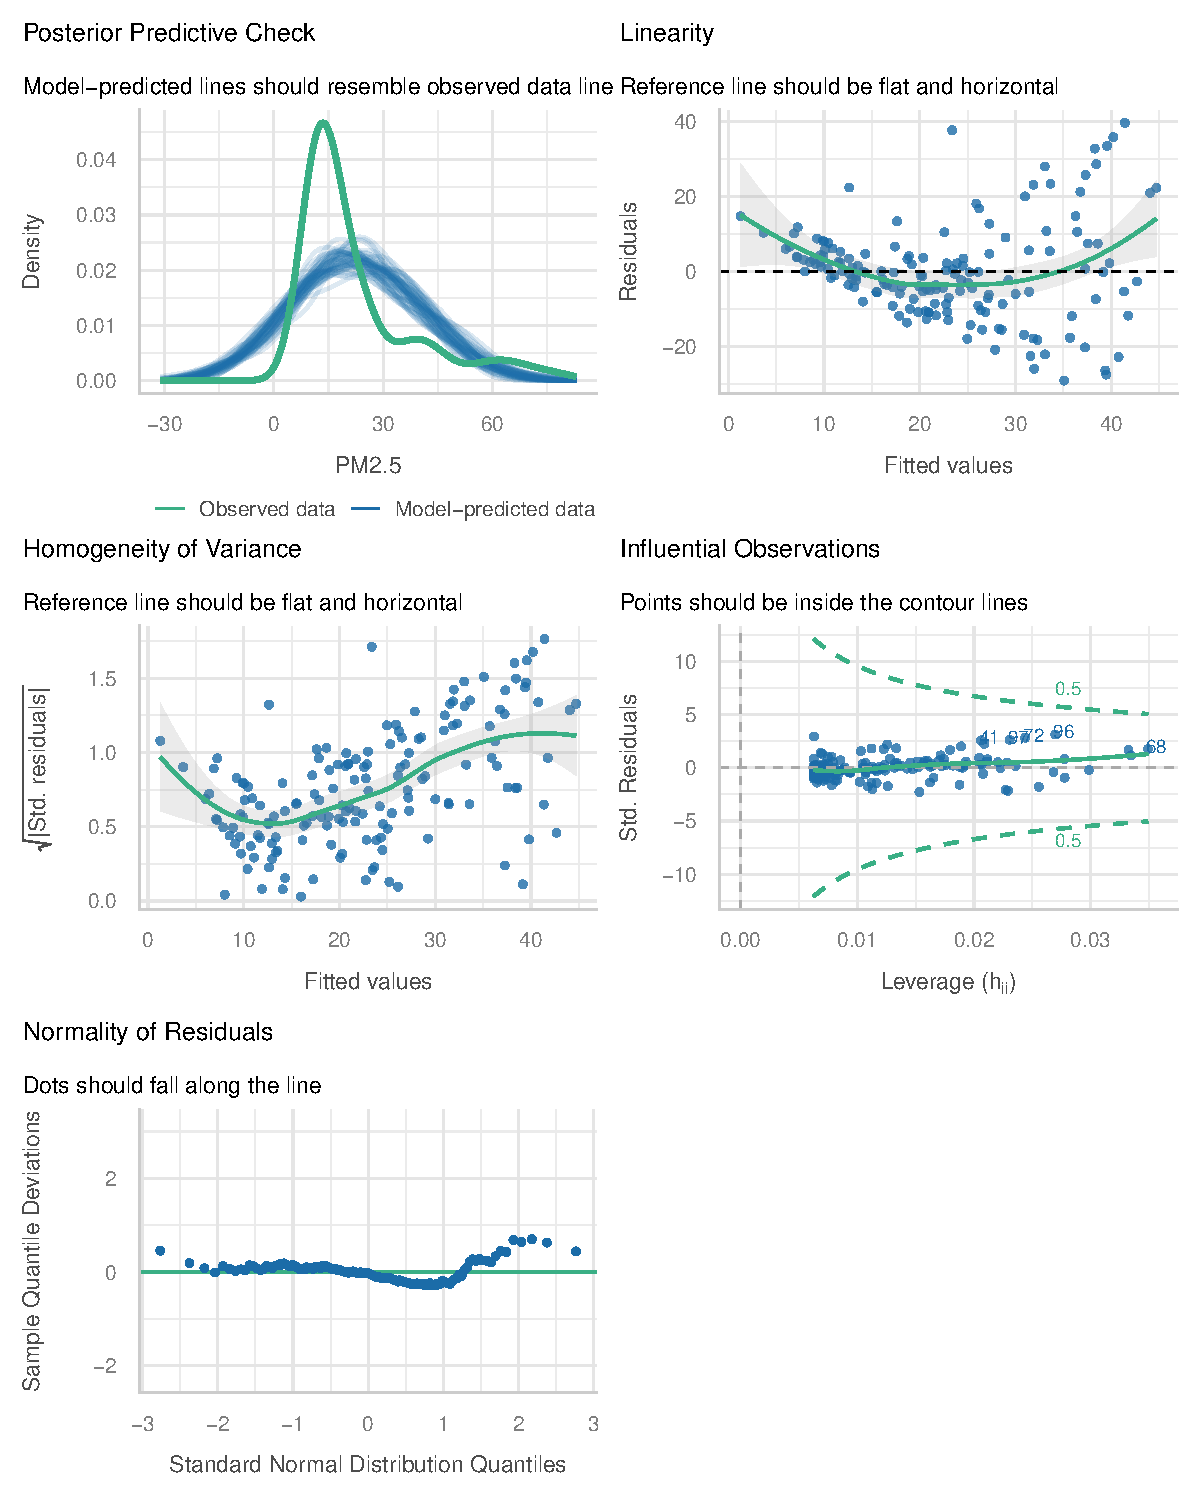
\includegraphics[width=0.9\linewidth,height=\textheight,keepaspectratio]{01-Informe_1_files/figure-latex/fig-diagnostico-met-1.pdf}

}

\caption{\label{fig-diagnostico-met}Diagnóstico de supuestos del MRLS
(PM2.5 \textasciitilde{} TMin)}

\end{figure}%

\subsection{Diagnóstico de supuestos MRLS con variable contaminante
(PM2.5 \textasciitilde{}
CO)}\label{diagnuxf3stico-de-supuestos-mrls-con-variable-contaminante-pm2.5-co}

\begin{figure}[H]

\centering{

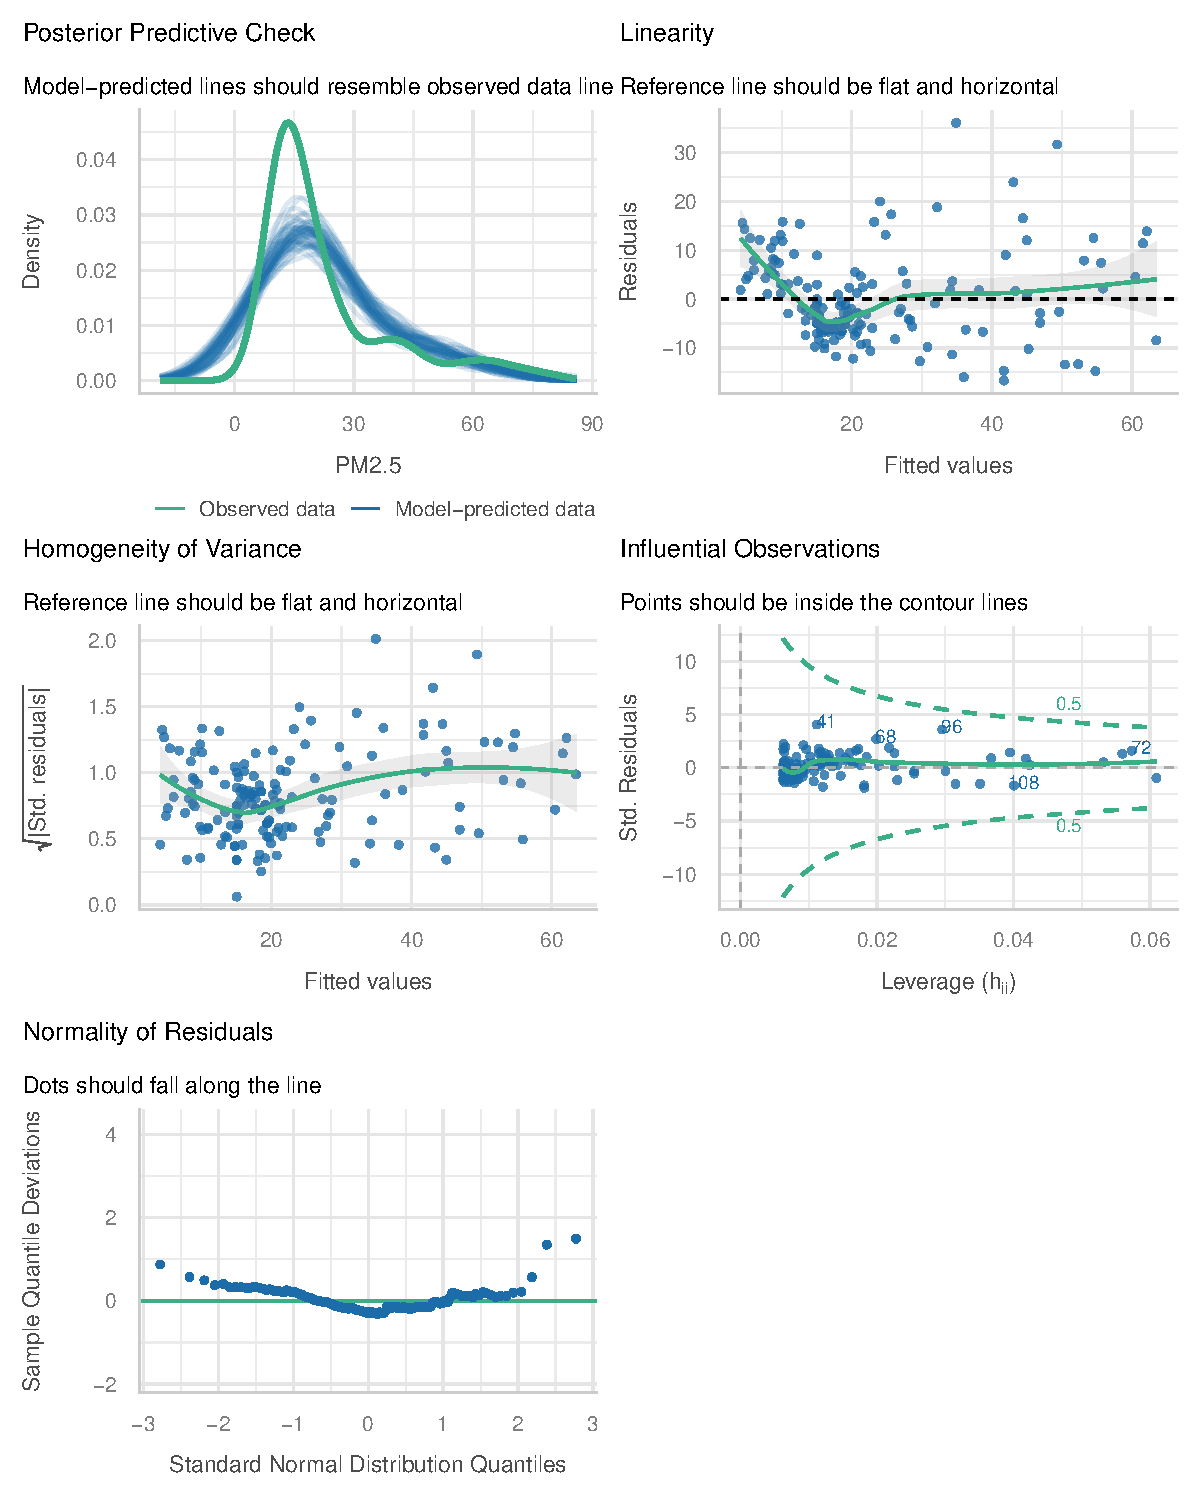
\includegraphics[width=0.9\linewidth,height=\textheight,keepaspectratio]{01-Informe_1_files/figure-latex/fig-diagnostico-cont-1.pdf}

}

\caption{\label{fig-diagnostico-cont}Diagnóstico de supuestos del MRLS
(PM2.5 \textasciitilde{} CO)}

\end{figure}%

\subsection{Pregunta 4. Diagnóstico de supuestos MRLM con una variable
metereológica y dos contaminantes (PM2.5 \textasciitilde{} TMin + NO2 +
CO)}\label{pregunta-4.-diagnuxf3stico-de-supuestos-mrlm-con-una-variable-metereoluxf3gica-y-dos-contaminantes-pm2.5-tmin-no2-co}

\begin{figure}[H]

\centering{

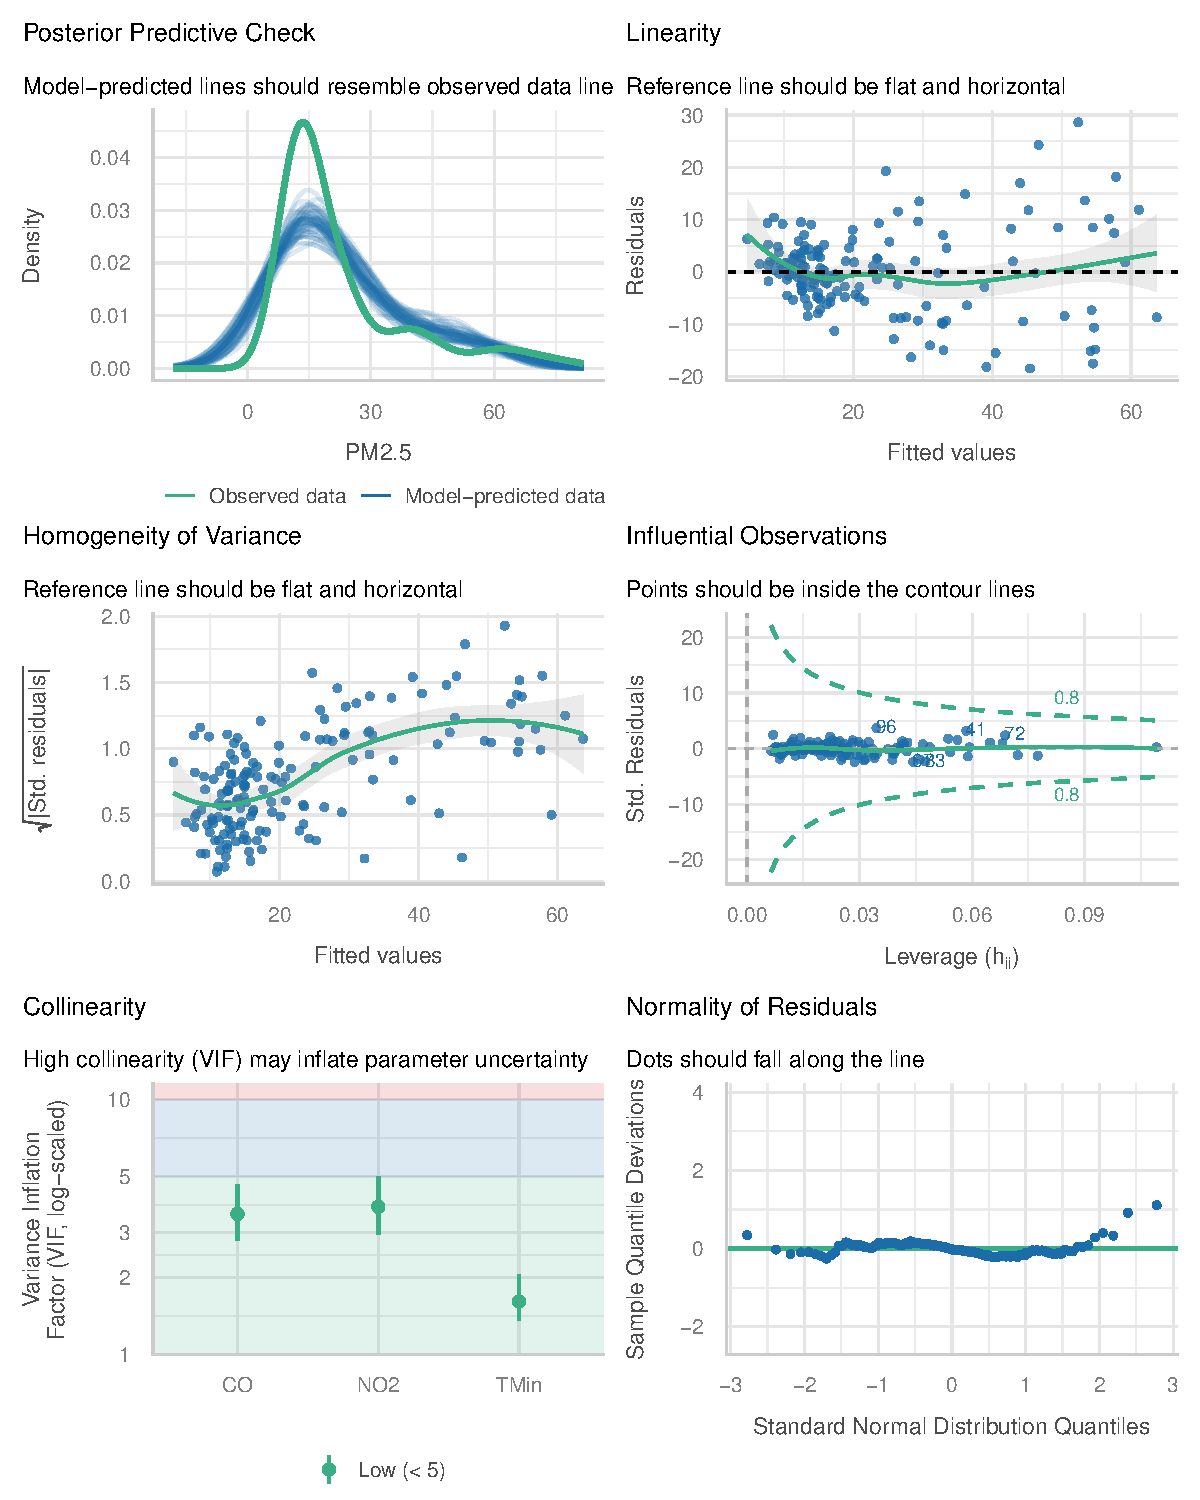
\includegraphics[width=0.9\linewidth,height=\textheight,keepaspectratio]{01-Informe_1_files/figure-latex/fig-diagnostico-mrlm-1.pdf}

}

\caption{\label{fig-diagnostico-mrlm}Diagnóstico de supuestos del MRLS
(PM2.5 \textasciitilde{} TMin + NO2 + CO)}

\end{figure}%




\end{document}
